% LaTex Template

\documentclass[12pt]{article}
\usepackage{natbib}
\usepackage[letterpaper, margin=1.1in]{geometry}
\usepackage{graphicx}
\usepackage{wrapfig}

\begin{document}
\noindent{Alexandra Pulwicki \\ \today}

\begin{center}
\Large \textbf{Colloquium Notes}
\end{center}



\noindent \textbf{Writing}
\begin{itemize}
\item Remove `temporal' from description of proposed research. Any temporal component would be an add-on to the project and not a major aspect
\item Make clear what was done in the past and what has yet to be completed (especially when discussing division of glaciers into regions)
\item Be more honest about why accumulation measurements are focused in the ablation area. Measurements in the accumulation area are too difficult and time consuming to accomplish with the proposed tools (probe). 
\item Differentiate between two components of the `point scale' 
\begin{itemize}
\item Taking $\sim$ 5 depth measurements at each sampling location $\rightarrow$ uncertainty for each depth measurement
\item Taking $\sim$ 125 depth measurements in a 40 x 40 m grid cell that corresponds to a DEM grid cell $\rightarrow$ uncertainty in snow depth for a DEM cell 
\end{itemize}
\item Clarify what is meant by `combinations of variables` (i.e. slope x orientation etc.)
\item Over emphasis on atmospheric rivers (too specific, might not even make it to the Yukon). Cyclones likely dominate precipitation patterns.
\item Resolution of atmospheric data is too low to make quantitative conclusions. Focus on a qualitative investigation of weather types and whether they are consistent with accumulation variability in Donjek Range
\item Correct grammatical mistakes identified throughout
\end{itemize}

\noindent \textbf{Figures}
\begin{itemize}
\item Include plots of glacier hypsometry
\item Compare mean slope vs centreline profile
\item Plot number of samples vs lag to examine distribution of measurements at all lag distances 
\end{itemize}

\pagebreak
\noindent \textbf{Clarifications}
\begin{itemize}
\item SWE variability in ablation area from \cite{McGrath2015}:

``Over the shortest spatial scales ($\sim$30--55 m) analyzed, SWE varies by up to 40\% of the local mean. The variability and, in particular, the relative variability, is greatest in ablation areas (Figure 8) and decreases at higher elevations. ... Enhanced variability in the ablation zone is consistent with large meter-scale surface roughness from crevasses, supraglacial streams, and moulins that characterize this zone. Wind redistribution of early season snowfall is preferentially deposited in surface depressions, thus smoothing the apparent surface roughness as the winter progresses, although the spatial pattern of the initial roughness is preserved in the end-of-season SWE \citep{Schirmer2011}. The observed variability in the ablation zone suggests that in order to accurately capture snow depth in this zone, one must average numerous sample points over a region approximately 30 x 30 m.''

\begin{figure}
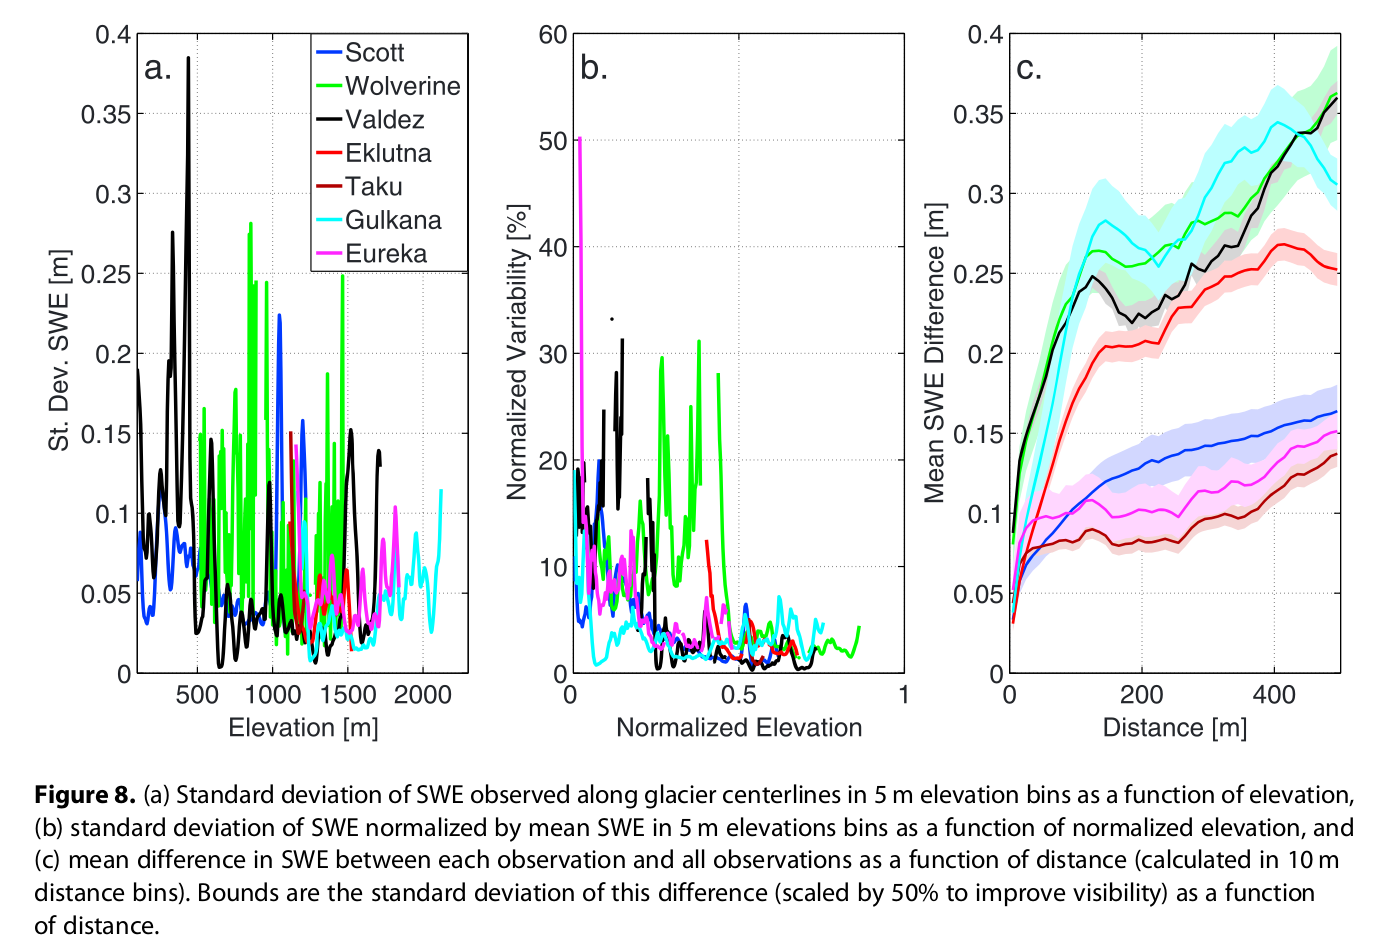
\includegraphics[width=\textwidth]{SWEablation.png}
\end{figure}

\end{itemize}

\noindent \textbf{Statistics Brain Storming}
\begin{itemize}
\item Create an outline of which statistical techniques will be used. Specify data/variables needed, equations, and metrics to evaluate outcome. 
\item Use measurement subsets to determine how `centered' a centre line transect should be. What affect does the location of a centre line transect have on the winter balance?
\item Compare various statistical characteristics between glaciers and see if they are transferable
\begin{itemize}
\item How does variability change with elevation (measurement standard deviation vs elevation plot)
\item Interpolation techniques (does each glacier have the same best technique?) 
\item Cross-glacier transects (variability across glacier)
\item Clustering of SWE
\end{itemize}
\item Propagation of error is important. \\
Measurement uncertainty $\rightarrow$ grid uncertainty $\rightarrow$ regression uncertainty $\rightarrow$ winter balance uncertainty
\item Challenge assumptions used in current methods of calculating winter balance by assessing errors. Going beyond basic statistics can set the new standard for how to obtain a more accurate estimate of winter balance and how to quantify uncertainty. 
\item When developing interpolation model, ensure that data is separated into calibration data, validation data, and testing data!
\item Use Monte Carlo simulation to create a distribution of winter balance estimates
\item Use \textbf{unbiased} standard deviation
\item Use R$^2$ to evaluate explained variance
\item Evaluate sensitivity of the regression to topographic parameters
\item Cluster snow depth data to determine grouping/zones that are present (compared to how we grouped them initatially). Can use hierarchical clustering of 3D plot (x, y, SWE)  to see how to divide glacier in the future and how this could help with future experimental design.
\item Do a SOM or PCA on variograms that are obtained at each measurement location. This could identify most characteristic variogram patterns and potentially identify variograms that correspond to different scales
\end{itemize}

\noindent \textbf{Other Thoughts}
\begin{itemize}
\item Is there a large volume of avalanched snow in the accumulation area due to increased precipitation on the higher elevation peaks adjacent to the accumulation area? Could this have an effect on the total accumulation in this area (indirect elevation effect)?
\item Is accumulation actually different in the accumulation and ablation areas or is it predominantly an elevation effect?
\end{itemize}


\bibliographystyle{igs}
\bibliography{MastersLit}

\end{document}



